\section{Future - Past}
The first logical check preformed on both the Sense2Vec and Word2Vec models was analysis of the future and past tense of a selection of verbs. The use path similarity between synsets in WordNet is used as a benchmark with any results featuring a similarity score, while this is an outdated method it further validates the power of vector models combined with cosine similarity.

\begin{table}[h]
\centering
\begin{tabular}{|l|r|r|r|}
\hline
\textbf{Future-Past} & \multicolumn{1}{c|}{\textbf{word2vec}} & \multicolumn{1}{c|}{\textbf{sense2vec}} & \multicolumn{1}{c|}{\textbf{WordNet}} \\ \hline
run - ran            & 0.44534984                             & 0.7623094                               & 1.0                                   \\ \hline
talk - talked        & 0.5017961                              & 0.72344923                              & 1.0                                   \\ \hline
see - seen           & 0.19250366                             & 0.48282138                              & 1.0                                   \\ \hline
have - had           & 0.6621415                              & 0.6477548                               & 1.0                                   \\ \hline
hold - held          & 0.28542474                             & 0.7731338                               & 1.0                                   \\ \hline
say - said           & 0.5547698                              & 0.68094736                              & 1.0                                   \\ \hline
lose - lost          & 0.5954038                              & 0.7762446                               & 1.0                                   \\ \hline
\end{tabular}
\caption{Future - Past Similarity}
\label{Future - Past Similarity}
\end{table}

\noindent
In the above table \ref{Future - Past Similarity} before comparing Word2Vec and Sense2Vec it is important to note all path similarity values for WordNet are = 1. WordNet in the case of tenses will resort the the base or present form of the verb, as such for "run - ran" the past tense will be queried as "run" giving a score of 1. This is actually a disadvantage of WordNet as storing of verbs in this form results in the loss of context. All words for the Sense2Vec query were tagged with the VERB POS tag and with Word2Vec just the word is supplied. When comparing the two vector systems used, for all comparisons Sense2Vec is much higher most notably with words that could be considered a noun or a verb depending on their context. For example "hold - held" could be interpreted as the verb to hold or the noun to have a hold of something. This idea of collision between verbs and nouns will be discussed further in section 4.2.

\section{Collisions}
Depending on the context of the word in a sentence a it may be interpreted as either a noun or a verb, the English language contains thousands of such words. Preforming a query to obtain the most similar vectors without the separation of verbs and nouns results in a loss of context with Word2Vec.

\begin{table}[h]
\centering
\begin{tabular}{|l|l|l|}
\hline
\multicolumn{3}{|c|}{\textbf{water}}                                                                                                  \\ \hline
\multicolumn{1}{|c|}{\textbf{word2vec}} & \multicolumn{1}{c|}{\textbf{sense2vec-VERB}} & \multicolumn{1}{c|}{\textbf{sense2vec-NOUN}} \\ \hline
seawater                                & mist                                         & silt                                         \\ \hline
groundwater                             & overwater                                    & sediment                                     \\ \hline
greywater                               & repot                                        & ocean                                        \\ \hline
rainwater                               & aerate                                       & chlorine                                     \\ \hline
effluent                                & soil                                         & evaporation                                  \\ \hline
potable                                 & fertilize                                    & submerged                                    \\ \hline
deionized                               & unpot                                        & liter                                        \\ \hline
moisture                                & replant                                      & water                                        \\ \hline
\end{tabular}
\caption{Collisions "Water" - Most Similar}
\label{Collisions "Water" - Most Similar}
\end{table}

\noindent
In table \ref{Collisions "Water" - Most Similar} Word2Vec returns the most similar vectors to "water" regardless of its context as such a list of mostly nouns are returned with some adjectives. When tagging "water" as a verb with Sense2Vec the majority of words returned are verbs and are relevant to the verb "to water". When tagged as a noun other nouns related to water are returned. 

\begin{table}[h]
\centering
\begin{tabular}{|l|l|l|}
\hline
\multicolumn{3}{|c|}{\textbf{sink}}                                                                                                   \\ \hline
\multicolumn{1}{|c|}{\textbf{word2vec}} & \multicolumn{1}{c|}{\textbf{sense2vec-VERB}} & \multicolumn{1}{c|}{\textbf{sense2vec-NOUN}} \\ \hline
explode                                 & float                                        & toilet                                       \\ \hline
sinks                                   & submerge                                     & bathtub                                      \\ \hline
submerge                                & submerse                                     & faucet                                       \\ \hline
capsize                                 & refloat                                      & tub                                          \\ \hline
penetrate                               & sail                                         & dishwasher                                   \\ \hline
overheat                                & evaporate                                    & washer                                       \\ \hline
drown                                   & swim                                         & bathroom                                     \\ \hline
scuttle                                 & capsize                                      & shower                                       \\ \hline
detonate                                & plunge                                       & commode                                      \\ \hline
evaporate                               & sunk                                         & washbasin                                    \\ \hline
\end{tabular}
\caption{Collisions "Sink" - Most Similar}
\label{Collisions "Sink" - Most Similar}
\end{table}

\noindent
Again in table \ref{Collisions "Sink" - Most Similar} there is a clear separation when tagging the word as a noun or a verb. With Word2Vec a list of relevant words are returned but are related to the verb "to sink", a similar list of words are returned from Sense2Vec when tagging it as a verb. However, greater context is obtained when looking at the word as a noun, the list contains object that are use water and these vectors are removed from the verb cluster of vectors.

\begin{table}[h]
\centering
\begin{tabular}{|l|l|l|}
\hline
\multicolumn{3}{|c|}{\textbf{fire}}                                                                                                   \\ \hline
\multicolumn{1}{|c|}{\textbf{word2vec}} & \multicolumn{1}{c|}{\textbf{sense2vec-VERB}} & \multicolumn{1}{c|}{\textbf{sense2vec-NOUN}} \\ \hline
fires                                   & shoot                                        & flame                                        \\ \hline
smoke                                   & eject                                        & lighting                                     \\ \hline
rhaptocarpa                             & firing                                       & blaze                                        \\ \hline
storm                                   & hire                                         & ablaze                                       \\ \hline
attack                                  & fireable                                     & alight                                       \\ \hline
bomb                                    & recock                                       & light                                        \\ \hline
firebomb                                & reload                                       & aflame                                       \\ \hline
blast                                   & fire                                         & wildfire                                     \\ \hline
shellfire                               & refire                                       & extinguisher                                 \\ \hline
gun                                     & fired                                        & extinguish                                   \\ \hline
\end{tabular}
\caption{Collisions "Fire" - Most Similar}
\label{Collisions "Fire" - Most Similar}
\end{table}

\noindent
Once again with table \ref{Collisions "Fire" - Most Similar} the Word2Vec column contains a mixture of verbs, nouns and adjectives. The noun section of Sense2Vec is made up of objects which would be related to a fire and as such these vectors are removed from the verb cluster of "fire". This results in the verb column containing actions relevant to the verb form of fire. 

It is important to note the most similar vectors returned by Sense2Vec for the verbs were other tenses of verb; these were removed to allow for a clearer compassion. Also some results were required to be removed do to misspelling, this could be rectified by the removing them during the parsing of the corpus or by avoiding the latest unreviewed articles added to Wikipedia.

\section{Verb to Verb Relations}
Next is a comparison of the present tense of two different verbs, specific verbs were chosen that may be used in similar contexts. Again WordNet's path similarity is used to obtain a benchmark against the two methods. With Sense2Vec all word are tagged using the VERB POS tag and just the words themselves are supplied to Word2Vec.

\begin{table}[h]
\centering
\begin{tabular}{|l|r|r|r|}
\hline
\multicolumn{1}{|c|}{\textbf{Verb to Verb}} & \multicolumn{1}{c|}{\textbf{word2vec}} & \multicolumn{1}{c|}{\textbf{sense2vec}} & \multicolumn{1}{c|}{\textbf{WordNet}} \\ \hline
lose - win                                  & 0.6463107                              & 0.57354873                              & 0.3333333333333333                    \\ \hline
shout - whisper                             & 0.59817475                             & 0.49780205                              & 0.3333333333333333                    \\ \hline
float - sink                                & 0.63962716                             & 0.5597029                               & 0.16666666666666666                   \\ \hline
borrow - lend                               & 0.6444298                              & 0.56534344                              & 0.2                                   \\ \hline
build - destroy                             & 0.574708                               & 0.339647                                & 0.2                                   \\ \hline
punish - reward                             & 0.38375688                             & 0.5213614                               & 0.1111111111111111                    \\ \hline
show - hide                                 & 0.25482053                             & 0.3824724                               & 0.25                                  \\ \hline
laugh - cry                                 & 0.60203165                             & 0.629749                                & 0.2                                   \\ \hline
\end{tabular}
\caption{Verb - Verb Similarity}
\label{Verb - Verb Similarity}
\end{table}

\noindent
With table \ref{Verb - Verb Similarity} initial inspection tends to show a higher similarity score for Word2Vec. However, the verb relations contain opposites which should produce a lower similarity score. With words used in similar contexts it would be difficult to get this score as low as WordNet but it appears that POS tagging has some influence in the reduction of the similarity score.

\section{Noun to Noun Relations}
Looking at noun to noun relations a similar approach was taken, however this time instead of using opposites a similar word which may be used in the same sentence was chosen. This choice was made due to more frequent use of nouns throughout a typical sentence. Once again the nouns are supplied to Word2Vec as is and tagged with the NOUN POS tag for Sense2Vec.

\begin{table}[h]
\centering
\begin{tabular}{|l|r|r|r|}
\hline
\multicolumn{1}{|c|}{\textbf{Noun to Noun}} & \multicolumn{1}{c|}{\textbf{word2vec}} & \multicolumn{1}{c|}{\textbf{sense2vec}} & \multicolumn{1}{c|}{\textbf{WordNet}} \\ \hline
laptop - music                              & 0.2156436                              & 0.27404207                              & 0.058823529411764705                  \\ \hline
car - drive                                 & 0.49729413                             & 0.34420764                              & 0.058823529411764705                  \\ \hline
window - house                              & 0.44160044                             & 0.36983767                              & 0.16666666666666666                   \\ \hline
actor - play                                & 0.23302217                             & 0.1917589                               & 0.07692307692307693                   \\ \hline
fire - water                                & 0.4858942                              & 0.3983069                               & 0.09090909090909091                   \\ \hline
work - pay                                  & 0.34210274                             & 0.3994102                               & 0.07142857142857142                   \\ \hline
\end{tabular}
\caption{Noun - Noun Similarity}
\label{Noun - Noun Similarity}
\end{table}

\noindent
In table \ref{Noun - Noun Similarity} for the majority of values Word2Vec obtains a higher similarity score. To incorporate POS tagging and the separation of words based on POS in the training process some relations are lost or reduced. For example words that can be interpreted as either a verb or a noun are now treated as separate vectors, resulting in a greater vocabulary size. This has its benefits as seen in table \ref{Collisions "Water" - Most Similar} but in turn comes with a reduction in context requiring a larger corpus to be used in training. The impacts of this will be discussed further in Chapter 5.

\section{Preposition to Preposition Relations}
The final POS comparison investigated was prepositions, WordNet is excluded from this set of results as it does not include prepositions in its vocabulary. As before the word is supplied to Word2Vec as is and tagged with the ADP tag.

\begin{table}[h]
\centering
\begin{tabular}{|l|r|r|}
\hline
\multicolumn{1}{|c|}{\textbf{Preposition to Preposition}} & \multicolumn{1}{c|}{\textbf{word2vec}} & \multicolumn{1}{c|}{\textbf{sense2vec}} \\ \hline
above - below                                             & 0.9064428                              & 0.7602379                               \\ \hline
inside - outside                                          & 0.7489509                              & 0.5698512                               \\ \hline
with - without                                            & 0.39408234                             & 0.13051958                              \\ \hline
up - down                                                 & 0.7235564                              & 0.3681819                               \\ \hline
before - after                                            & 0.9362761                              & 0.70483726                              \\ \hline
against - for                                             & 0.4246056                              & 0.21836904                              \\ \hline
\end{tabular}
\caption{Preposition - Preposition Similarity}
\label{Preposition - Preposition Similarity}
\end{table}

\noindent
In the above table \ref{Preposition - Preposition Similarity} the opposite form of each is compared similar to verb relations in table \ref{Verb - Verb Similarity}. Once again a lower score is expected but still increased due to opposites being used in similar contexts. The similarity score is substantially lower for some examples such as "up - down" however which system is favoured would be entirely based on the use case.

\section{Synset Similarity}
As discussed to validate the above results some statistical methods were introduced, the first of which is analysis of the similarity between 1000 randomly selected nouns and verbs. A verb is selected at random and its synsets are obtained from WordNet, a similarity comparison of the random word and the following is conducted using both Word2Vec and Sense2Vec:
\begin{itemize}
  \item The first word from the first synset
  \item The last word from the first synset
  \item The last word from the last synset
\end{itemize}

\begin{figure}[H]
\centering
  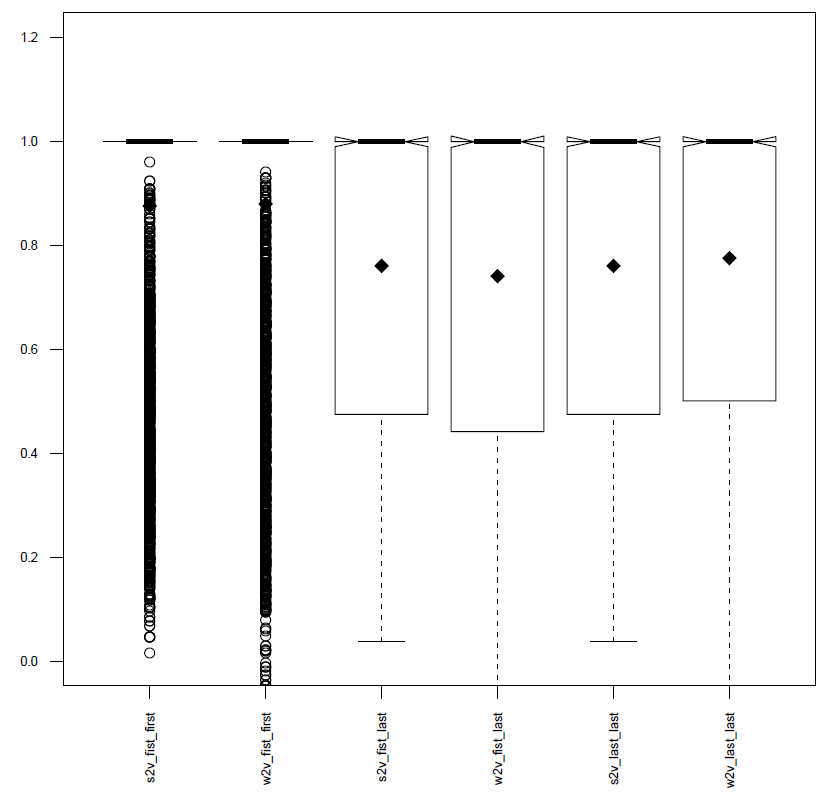
\includegraphics[width=\textwidth]{images/wordnet_nouns.PNG}
  \caption{Synset Comparison Nouns}
  \label{fig:wordnet_nouns}
\end{figure}

\noindent
In the figure \ref{fig:wordnet_nouns} the majority of the time the first word in the first sysnet is the word supplied itself, resulting in a similarity score of 1. The median values for both Sense2Vec and Word2Vec tend to be similar in figure \ref{fig:wordnet_nouns} However the outlier tails tend to be longer with Word2Vec.

\begin{figure}[H]
\centering
  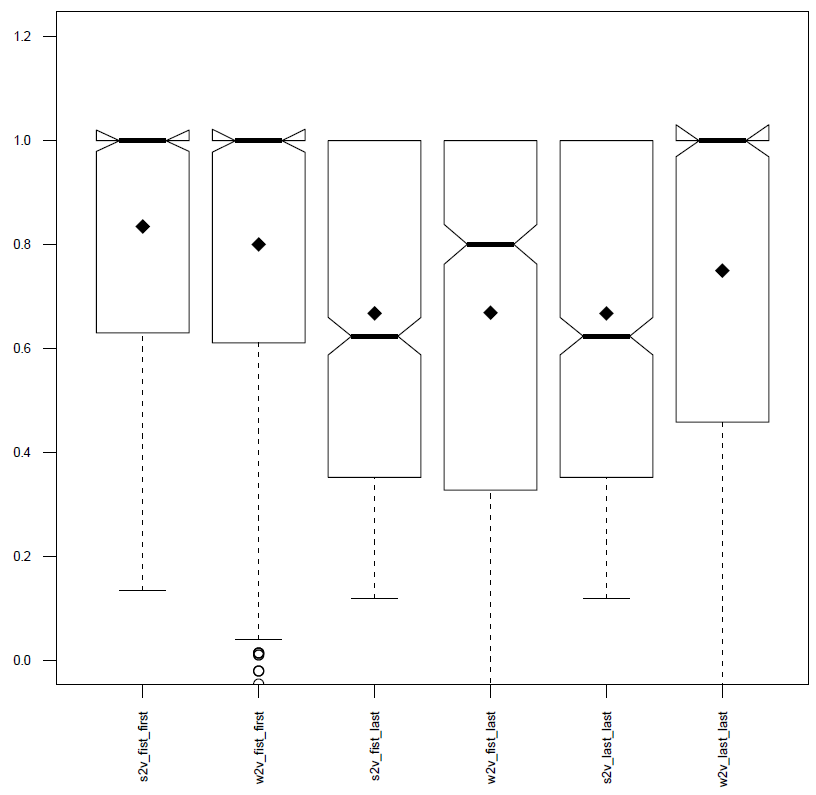
\includegraphics[width=\textwidth]{images/wordnet_verbs.PNG}
  \caption{Synset Comparison Verbs}
  \label{fig:wordnet_verbs}
\end{figure}

\noindent
Looking at the analysis of verbs in figure \ref{fig:wordnet_verbs} once again the tail of outliers and the max value for Word2Vec is higher. There is a high positive skew in the first two plots again due to the high number of exact matches. However Word2Vec for the rest of the groups has a large positive skew towards 1. With Sense2Vec the similarity drops with a slight negative skew which is expected as we progress further down and across the synsets.

With the above two plots \ref{fig:wordnet_verbs} and \ref{fig:wordnet_nouns} no median lies outside of Q1 or Q3 so it can not be said with confidence that the two methods are unique. However due to the high concentration of exact matches, the resulting data is left to be treated as outliers and pushed outside of Q3.

\section{Bloom's Taxonomy}
To attempt to show clear distinction between the two methods further analysis was completed using Bloom's Taxonomy as a basis. Similarity values are obtained between each verb in each level of the taxonomy excluding the verb itself ($n^2-n$ comparisons for each category). The verb was supplied to Word2Vec as is and tagged with the VERB POS tag for Sense2Vec, each level in the taxonomy was given its own boxplot.

\begin{figure}[H]
\centering
  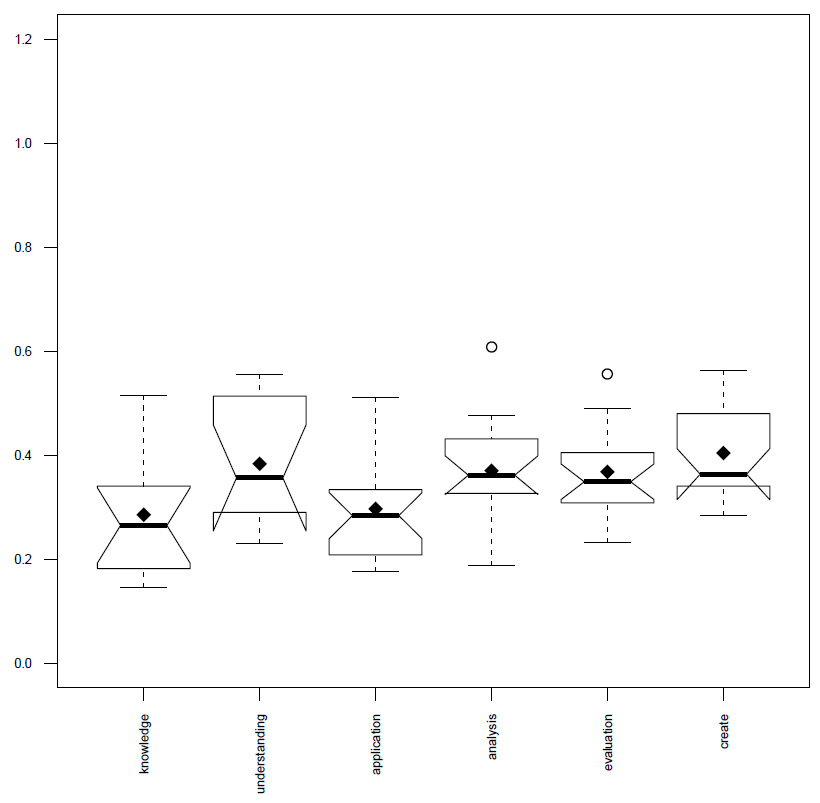
\includegraphics[width=.9\textwidth]{images/s2v_bloom.PNG}
  \caption{Sense2Vec Bloom's Taxonomy}
  \label{fig:bloom_s2v}
\end{figure}

\noindent
For Sense2Vec in figure \ref{fig:bloom_s2v} all levels form a condensed interquartile range with few outliers. In the lower 3 levels; create, evaluation and analysis the median of each lies within the interquartile range of the next showing there is a consistency in similarity score across the categories.

\begin{figure}[H]
\centering
  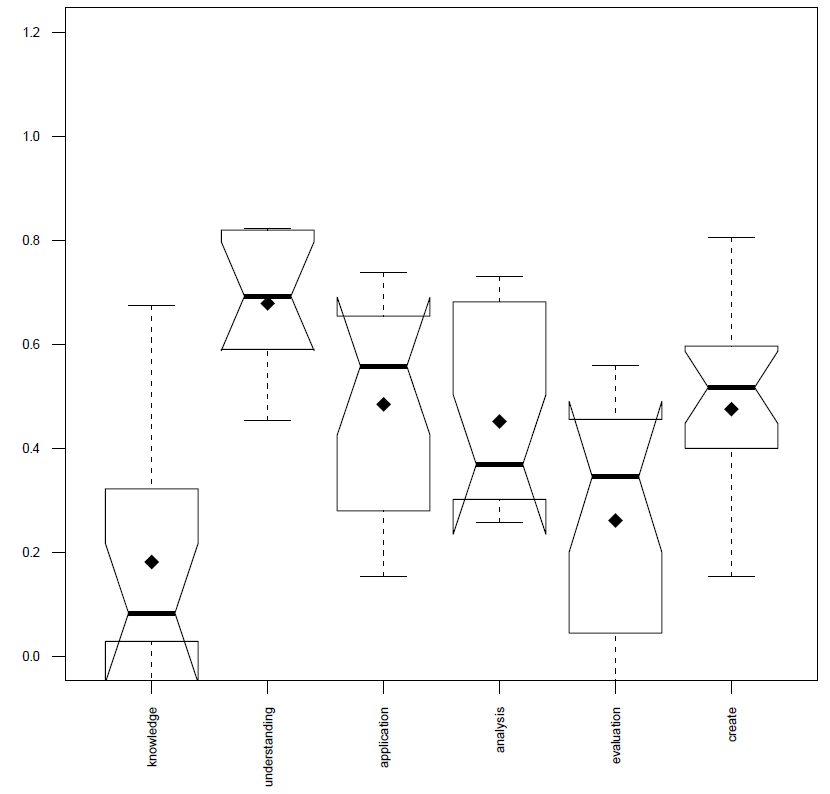
\includegraphics[width=\textwidth]{images/w2v_bloom.PNG}
  \caption{Word2Vec Bloom's Taxonomy}
  \label{fig:bloom_w2v}
\end{figure}

\noindent
When looking at Word2Vec in figure \ref{fig:bloom_w2v} the interquartile range is much less condensed and with the create category much more values are found outside the interquartile range. The the median of the knowledge category lies well outside the interquartile range of the next category understanding, showing a lack of consistency of similarity score across the levels. While the median of the plots for Word2Vec is closer to 1 in two levels and positively skewed towards on in two others, this is negated by the lack of consistency across the levels with Word2Vec producing a low interquartile range for the knowledge and evaluation levels.

\begin{figure}[H]
\centering
\begin{minipage}{.5\textwidth}
  \centering
  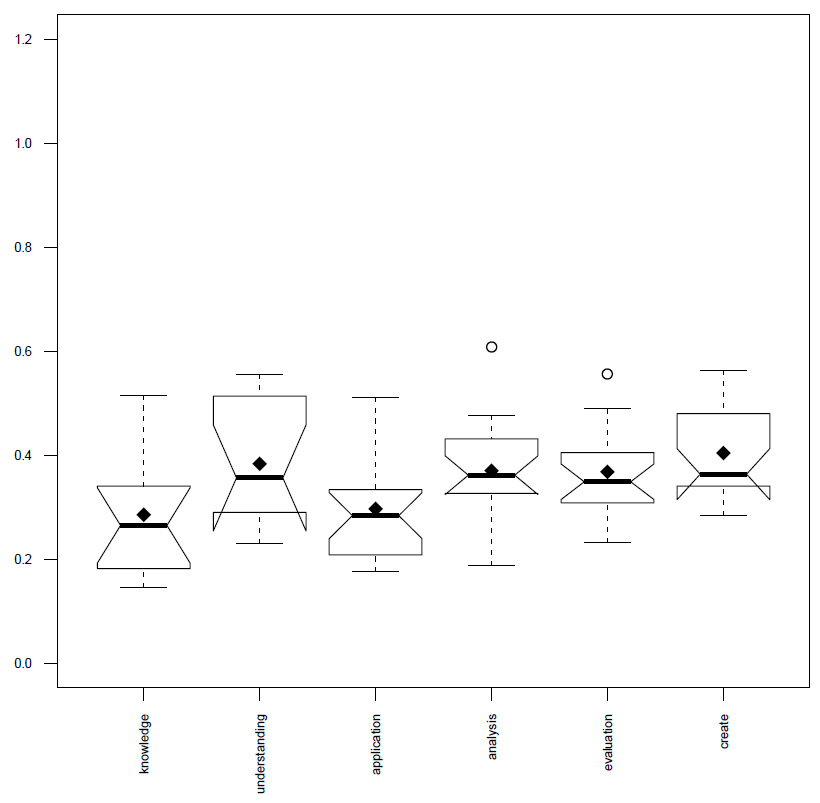
\includegraphics[width=1\linewidth]{images/s2v_bloom.PNG}
  \caption{(a) Sense2Vec}
  \label{fig:s2v}
\end{minipage}%
\begin{minipage}{.5\textwidth}
  \centering
  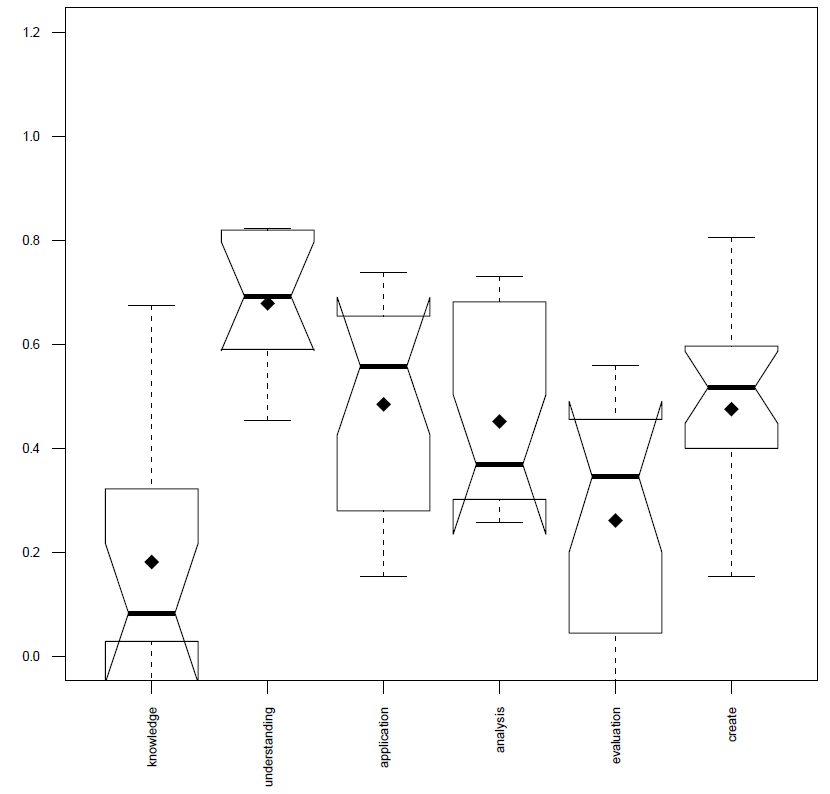
\includegraphics[width=1\linewidth]{images/w2v_bloom.PNG}
  \caption{(b) Word2Vec}
  \label{fig:w2v}
\end{minipage}
\caption{Side By Side Comparison}
\label{fig:side_by_side}
\end{figure}

\noindent
Finally looking the side by side comparison in figure \ref{fig:side_by_side} some distinction can be made between the two methods. For all levels except analysis and understanding the median in figure \ref{fig:w2v} is well outside the interquartile range and in some cases the max value of the corresponding level in figure \ref{fig:s2v}. Sense2Vec appears to show a more consistent similarity score across the six levels, Word2Vec's similarity score tends to fluctuate dramatically with a large difference between the first two levels on the plot in figure \ref{fig:w2v}. Also of note is the max value of both methods, for Sense2Vec the max and mix values are much smaller with fewer values outside the interquartile range. With Word2Vec the opposite is true not only is the interquartile range spread over a larger range of values but also the values outside this range extend further than that of Sense2Vec.